\documentclass[a4paper,14pt]{extarticle} \usepackage[utf8]{inputenc}
\usepackage[T1]{fontenc}
\usepackage[margin=2.5cm]{geometry}

% Fonte Caladea se existir, senão lmodern
\IfFileExists{caladea.sty}{
  \usepackage{caladea}
}{
  \usepackage{lmodern} }
\usepackage{ragged2e}
\usepackage{graphicx}
\usepackage[portuguese]{babel}
\usepackage{wrapfig}
\usepackage{hyperref}
\usepackage{fancyhdr}
\usepackage{xcolor}
\usepackage{rotating}
\usepackage{titlesec}
\usepackage{epigraph}
\usepackage{dirtytalk}
\usepackage{indentfirst} % Indenta o primeiro parágrafo após seções

% Ajuste do recuo de parágrafo
\setlength{\parindent}{1.5em}

% Centralizar títulos
\titleformat{\section}
  {\normalfont\centering\bfseries\Large}{}{1em}{}

\titleformat{\subsection}
  {\normalfont\centering\bfseries\large}{}{1em}{}

\titleformat{\subsubsection}
  {\normalfont\centering\bfseries}{}{1em}{}

% -------------- Símbolos de Versículo e Resposta --------------
% Definição do símbolo (a “barrinha” inclinada)
\makeatletter
\newcommand{\vers@resp@sym}{%
  \raisebox{0.2ex}{\rotatebox[origin=c]{-20}{$\m@th\rceil$}}%
}
% macro interna que sobrepõe a barrinha e a letra V ou R
\newcommand{\vers@resp}[2]{%
  {\ooalign{%
     \hidewidth\kern#1\vers@resp@sym\hidewidth\cr
     #2\cr
  }}%
}
% comandos públicos \versicle e \response
\DeclareRobustCommand{\versicle}{\vers@resp{-0.1em}{V}}
\DeclareRobustCommand{\response}{\vers@resp{0pt}{R}}
\makeatother
% ^------------- Símbolos de Versículo e Resposta -------------^

% Rodapé com imagem e página
\pagestyle{fancy}
% ---- Cabeçalho ------------
\fancyhf[C]{}
% ----- Rodapé --------------
\fancyfoot[LO,LE]{%
  
\includegraphics[scale=0.2]{assets/cross.png}\quad
  \textit{\textit{Santa Mãe de Deus, Rogai por nós.}}
}
\fancyfoot[RO,RE]{\thepage}

\usepackage{pdfpages}
\begin{document}
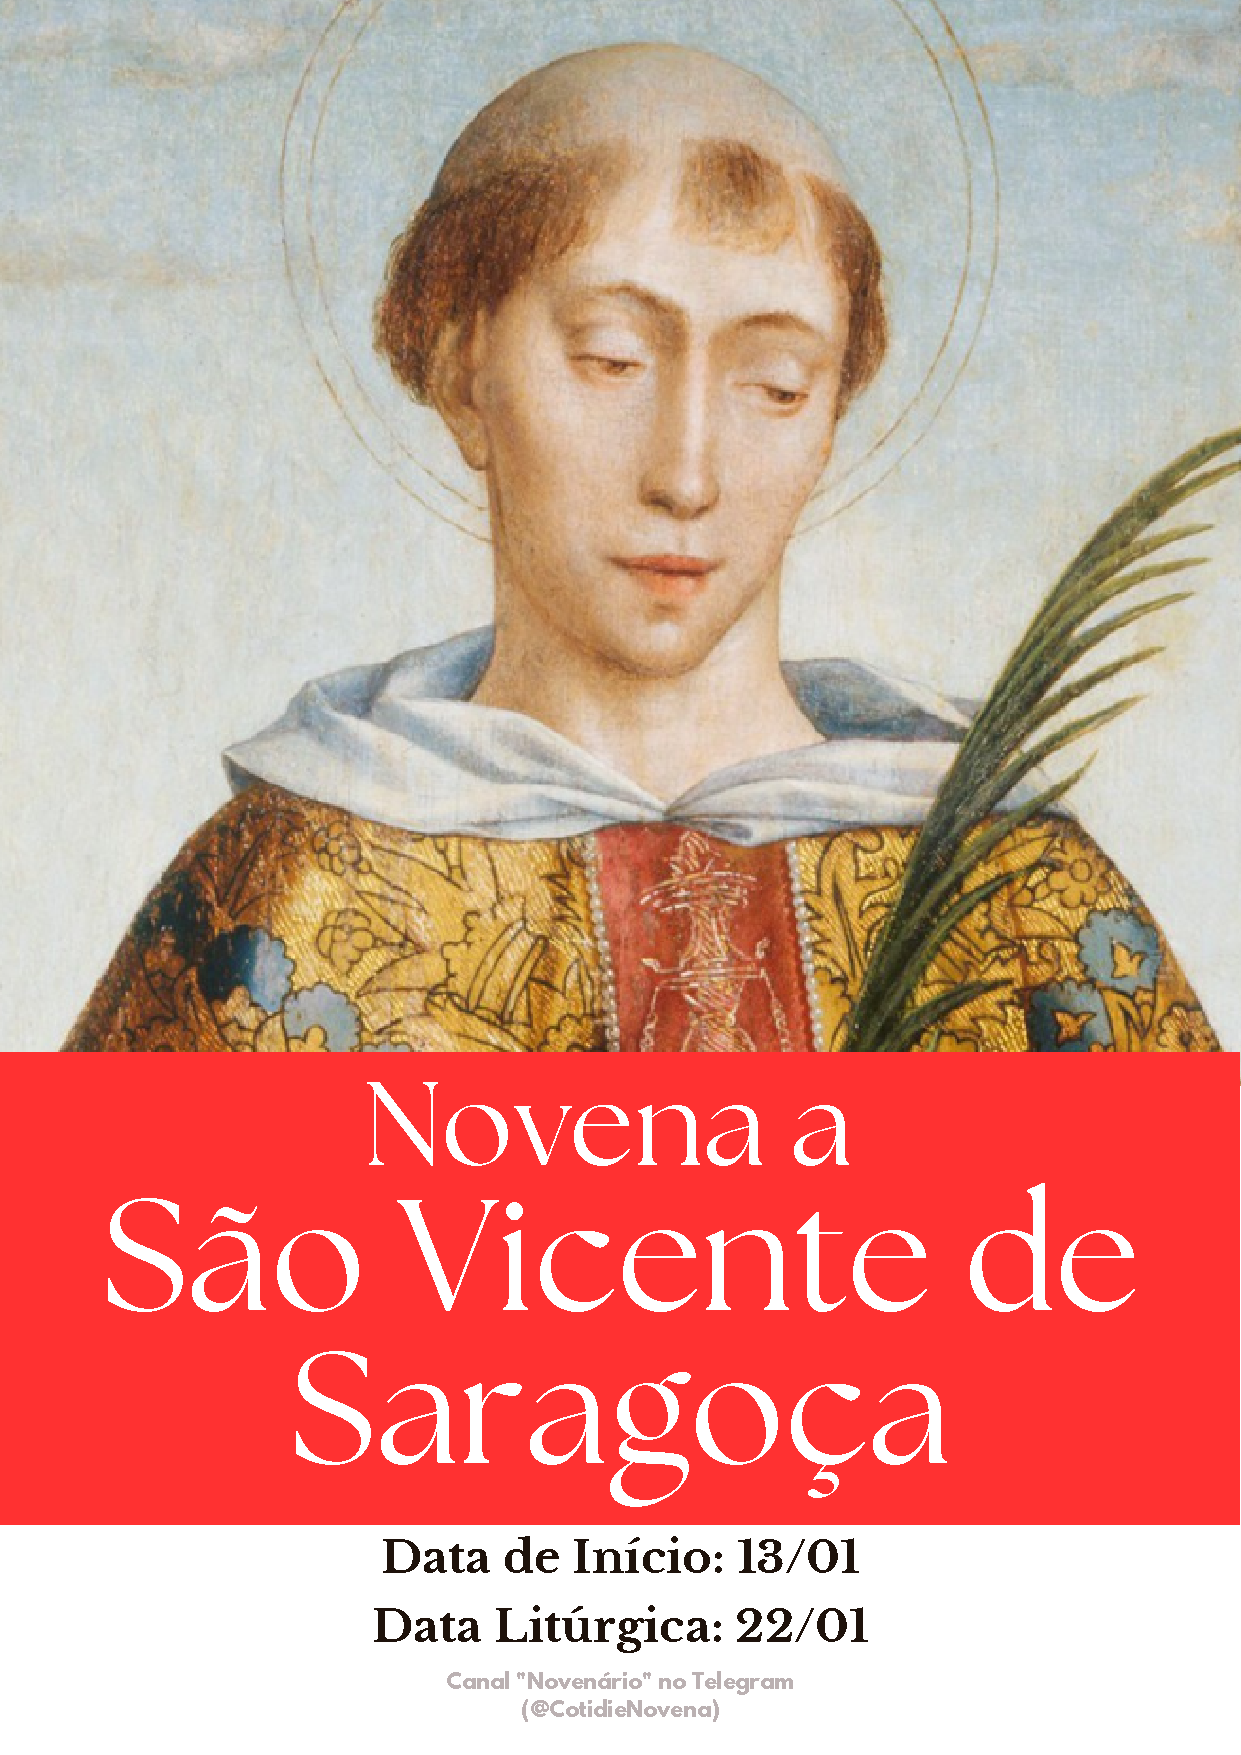
\includepdf[pages=1]{Capa São Vicente de Saragoça}


\begin{center}
  {\huge Novena de São Vicente de Saragoça}
\end{center}



\noindent\rule{\textwidth}{0.4pt}
\tableofcontents
\thispagestyle{empty}


% --- História ---

\section{História}

São Vicente foi um dos mais célebres mártires da Espanha. Nascido em Saragoça, de uma das melhores famílias daquela cidade, desde a sua juventude foi colocado sob a direção de Valério, bispo daquela igreja, que o instruiu com abundância nos dogmas da religião e também nas humanidades. Como Vicente se tornasse muito sábio, Valério ordenou-o diácono; e por ter o prelado uma limitação na fala, deu-lhe a missão de pregar. E o nosso santo cumpriu bem o seu ofício, convertendo grande número de pecadores, e até de pagãos.

Naquele tempo, ou seja, no ano 103, as Espanhas estavam sob o domínio de Maximiliano, e Daciano era governador da província de Tarragona, na qual estava Saragoça. Daciano foi um homem crudelíssimo e grande inimigo dos cristãos; por isso, quando soube dos grandes êxitos que Vicente obtinha em prol da religião cristã, ordenou que ele e seu bispo Valério viessem até Valência, onde ele residia. 

Primeiro, fê-los sofrer muito na prisão, para que os maus tratos os tornassem mais suscetíveis a perverter-se. Mas rapidamente ele percebeu que esse meio pouco ajudaria no seu intento. Depois, mandando que se apresentassem diante dele, a princípio falou-lhes com doçura: a Valério, disse que sua idade avançada lhe pedia descanso, coisa que ele certamente encontraria se obedecesse às ordens do imperador; e voltando-se a Vicente, disse: “Vós sois jovem. Esperai os favores da sorte que se vos apresenta; para os merecer, bastará que abandoneis a vossa religião. Meu filhinho, obedecei ao imperador e não vos exponhais, recusando, a uma morte ignominiosa”.
“São Vicente Mártir”, por Urbano Fos.

Então Vicente se voltou para Valério, que nada havia respondido às palavras do governador, e disse-lhe: “Ó pai, se vos aprouver, responderei eu em vosso lugar”. O santo bispo, disposto já a sofrer tudo por Jesus Cristo, respondeu-lhe: “Sim, filho, assim como vos encarreguei de pregar por mim a Palavra de Deus, assim também agora vos encarrego de proclamar a nossa fé”. Declarou Vicente então a Daciano que eles não adoravam mais que a um só Deus, não podendo adorar os demônios, que eram os deuses do império. E acrescentou: “Além disso, não creiais que tendes o poder de nos abalar com ameaças de morte ou promessas de honras, porque nada há no mundo que se compare à honra e ao prazer que encontramos em morrer por Jesus Cristo”. 

Daciano, irado diante da liberdade com que lhe falou o santo diácono, disse com furor: “Ou ofereceis incenso aos deuses, ou pagareis com a morte o desprezo que demonstrais”. E São Vicente, elevando a voz, respondeu: “Já vos disse ser este o maior prazer e honra que nos podeis fazer: o de morrer por Jesus Cristo. E ficai certo de que mais rápido vos cansareis de atormentar-nos do que nós de sofrermos os tormentos [que nos infligirdes]”.

Então, Daciano mandou Valério para o exílio e pôs-se a descarregar sobre Vicente toda a sua cólera. Primeiro, amarrou-o sobre um cavalete, onde foram de tal modo esticados suas mãos e os seus pés com aquela máquina hedionda, que imediatamente se ouviram os seus ossos sendo deslocados, não ficando os membros do santo unidos senão por meio dos nervos. Vendo, porém, o tirano a placidez do santo naqueles tormentos, e ouvindo de sua boca: “Eis o que eu sempre desejei que acontecesse comigo, eis o fim dos meus suspiros”, livrou-se ele dos algozes e fez com que lhes batessem com varas, pensando que era por culpa deles o santo não sentir os golpes [que lhe davam]. 

Depois, ordenou que lhe dilacerassem o dorso e os lados com pregos de ferro, até que suas costas ficassem na carne viva. Sabendo o quanto cresce a dor das feridas quando reabertas depois de terem arrefecido, mandou que os flancos fossem de novo rasgados com pregos; e isto até que viessem à tona as vísceras do santo, com o sangue fluindo como um riacho. Mas mesmo aí Vicente insultava o governador, dizendo-lhe: “Já que os vossos ministros não têm força, por que não vindes vós, que sois o principal carrasco, em auxílio deles? Ponde também vós as mãos em mim e saciai a vossa sede no meu sangue! Vós vos enganais, se pensais que me vencereis com os tormentos; dentro de mim há um outro homem, sustentado por Deus, que vós não podeis vencer”. 
“São Vicente de Saragoça”, por Tomás Giner.

Vendo a sua constância, disse-lhe o tirano: “Ao menos, ao menos entregai-me os livros sagrados que guardais, para que eu os possa atirar ao fogo”. Ao que respondeu São Vicente que o fogo servia não para queimar os livros sagrados, mas para castigar eternamente os ímpios; e não hesitou em alertá-lo: se ele não abandonasse o culto dos ídolos, um dia, ele seria condenado eternamente a esse fogo.

Sentindo-se insultado pela resposta, o governador ficou furioso e condenou-o a ser queimado numa grelha de ferro toda armada com pontas afiadas. Ouvindo a ordem bárbara ser dada, São Vicente adiantou-se aos carrascos e subiu ele mesmo sobre a grelha, onde o fogo já ardia por baixo, deixando que lhe acorrentassem as mãos e os pés. Enquanto as brasas o torravam, os algozes aplicavam lâminas vermelhas quentes na carne lacerada de seu peito e de sua barriga. Por fim, atiraram pedaços de sal sobre as feridas, que caíam no fogo e depois subiam violentamente na direção de sua carne toda queimada e rasgada.

Entretanto, em meio àqueles tormentos, Vicente se apresentava com o rosto sorridente e com os olhos voltados para o Céu, bendizendo o Senhor, que aceitava o seu sacrifício. Todos admiravam a força prodigiosa que Deus comunicava ao santo jovem, e os próprios pagãos gritavam: “Milagre! Milagre!” Por isso, Daciano foi obrigado a afastar da vista do público aquele espetáculo de paciência. Ordenou que Vicente fosse conduzido ao cárcere, onde, não contente com as tantas torturas que lhe havia feito, quis [ainda] que lhe fossem amarrados os pés em cepos de madeira (um instrumento brutal chamado nervo, no qual vários santos confessores perderam a vida); mandou também que fosse deitado de costas sobre muitos cacos de vasos quebrados, os quais lhe abriram de novo as feridas com as pontas afiadas, provocando nele uma dor agudíssima. 

Ordenou, ademais, a fim de cansar a paciência do santo, que ninguém se aproximasse dele para dizer qualquer palavra de conforto; mas Deus tornou vãos os seus planos, pois Ele mesmo veio consolar o seu servo, chamando-o ao paraíso. Nas profundezas da noite, viu o santo um grande esplendor; viu também se soltarem os seus pés dos lenhos que os prendiam, e ao mesmo tempo sentiu-se revigorado por uma visita celeste: muitos anjos vieram até ele, da parte de Jesus Cristo, e anunciando-lhe o fim de suas penas, convidaram-no a tomar parte na glória do Céu. Os guardas, acordados pelos raios daquela luz que atravessava as fendas da porta, aproximaram-se dela e, tendo ouvido os anjos unidos louvar a Deus com o mártir, abraçaram todos a fé cristã. 

Informado de tudo isso, Daciano ordenou que tirassem Vicente da prisão, que o deitassem em uma cama macia e que lhe tratassem as feridas, a fim de que, restaurado, ele pudesse encarar novos tormentos. Avisados disso, os fiéis correram para visitar o santo e aliviá-lo: uns lhe beijavam as chagas, outros as enxugavam com panos, para depois as guardar como joias [preciosas] em casa. Mas, chegada finalmente para Vicente a hora do triunfo, suspirou ele sobre aquele leito entre os abraços de seus irmãos e à vista dos anjos, que o assistiram e depois o acompanharam até o Reino bem-aventurado.
“Morte de São Vicente”, pelo Mestre de Castelsardo.

Ouvindo falar de sua morte, mandou o tirano que o corpo do santo fosse deixado exposto aos animais, para lhes servir de alimento. Mas o Senhor providenciou um corvo, que, com as garras e o bico, defendeu-o dos outros bichos, especialmente de um lobo que tinha vindo devorá-lo. Daciano, não sabendo mais o que fazer contra o santo, ordenou que seu corpo fosse encerrado num saco e atirado ao mar. A ordem foi obedecida, mas o saco, mesmo amarrado a uma grande pedra, ficou flutuando como uma pena sobre as águas, e o vento o empurrou em direção a Valência: os marinheiros se esforçaram para alcançá-lo, mas, antes que eles chegassem, as ondas depositaram o corpo do santo na praia, onde de súbito ele foi coberto pela areia. 

Apareceu então o santo a uma piedosa mulher chamada Jônica e mostrou-lhe o lugar onde estava o seu corpo. Depois, foi ela de imediato com os outros cristãos [ao local] e, encontradas aquelas sagradas relíquias, depositaram-nas por um tempo numa pequena igreja; porém, feitas as pazes [do império] com a religião, transportaram-se as relíquias a um templo magnífico perto de Valência, onde elas são sempre veneradas com grande devoção. 

[Sobre São Vicente] escreve Santo Agostinho: “Que reino há hoje que goze do nome cristão e não se alegre em celebrar o nascimento de Vicente [para o Céu]?”. Os atos do martírio deste grande santo foram transcritos também por Ruinart.

% --- Orações Diárias ---
\newpage


\vfill

\section{Orações}

\subsection{Orações Para Todos os Dias}

Senhor Deus, que fortalecestes São Vicente de Saragoça em meio às torturas e perseguições do século IV, concedei-nos, por sua intercessão, a graça de permanecermos fiéis à Vossa verdade. Este diácono, que serviu com devoção ao lado de São Valério, enfrentou o governador Daciano com uma coragem que só pode vir de um coração totalmente entregue à Vossa vontade. Sua firmeza diante do sofrimento é um testemunho eterno de que o amor a Cristo triunfa sobre qualquer adversidade.

Ó São Vicente, vosso exemplo nos ensina que a verdadeira liberdade encontra-se na obediência a Deus, mesmo quando isso significa enfrentar os poderes deste mundo. Inspirai-nos a viver com a mesma determinação que sustentou vossa alma durante os tormentos, para que, em nossa fraqueza, possamos encontrar força no Espírito Santo. Assim como vosso sangue foi semente de novos cristãos, fazei que nossos sacrifícios diários sejam oferta viva em favor da salvação do próximo.

Senhor, pela intercessão de São Vicente, ajudai-nos a testemunhar Vosso amor com coragem e constância, para que, ao fim de nossa peregrinação terrena, sejamos acolhidos na glória eterna. Por Jesus Cristo, Vosso Filho, na unidade do Espírito Santo. Amém.

\[\textbf{Pai-Nosso, Ave-Maria, Glória-ao-Pai...}\]

\vfill

\begin{center}
\subsection*{Fontes:}
Adaptado de: {\color{blue} \underline{\href{https://www.praymorenovenas.com/holy-spouses-novena}{Pray More Novenas}}} e {\color{blue} \underline{\href{https://cruzterrasanta.com.br/sao-vicente-de-saragoca/540/105/}{Cruz Terra Santa}}}
\end{center}


\end{document}
